\documentclass[conference]{IEEEtran}

\usepackage[utf8]{inputenc}
\usepackage[T1]{fontenc}
\usepackage{amsmath}
\usepackage{graphicx}
\usepackage{cite}
\usepackage{url}
\usepackage[caption=false,font=footnotesize]{subfig}
\usepackage{xspace}
\usepackage[draft,inline,nomargin,index]{fixme}
\fxsetup{theme=color}
\usepackage{comment}

\begin{document}

\title{Implementing Virtual Synchrony in a P2P group communication}

\author{
	\IEEEauthorblockN{Piermaria Arvani, S198465, \texttt{piermaria.arvani@studenti.unitn.it}}
	\IEEEauthorblockN{Lorenzo Brugnera, S197054, \texttt{lorenzo.brugnera@studenti.unitn.it}}
}

\maketitle

\begin{abstract}
The project consists of developing a distributed application using Akka \cite{Akka}. The actors taking part in the system are called Akka actors and they are able to exchange messages between each other under some conditions/restrictions. Each peer is both able to send and deliver multicast messages and the overall system is fault tolerant in case of silent crash of a group member. The main purpose of this work is to implement the virtual synchrony guarantees.

\begin{comment}
	Quickly describe what your work is about, what you have been doing, what are the main conclusions.
The abstract is normally present in long reports, if your report is 1--3 pages you can avoid it as reading the entire document is not a major effort. 
\end{comment}
\end{abstract}

\section{Introduction}
\label{sec:introduction}
The project aims at showing a simple message exchange mechanism between
peers belonging to the same group. The actors taking part in the group
are of two types:
\begin{itemize}
	\item \textbf{Manager}
	\item \textbf{Participant}
\end{itemize} 
There is only one group manager, it is reliable, responsible for serializing group view
changes and sending view updates to all the participants. Furthermore, it is also able to detect silent crashes and initiate view changes to notify the other members that the group has changed.

The exchange of messages is governed by the \texttt{Virtual Synchrony} protocol, which ensures on one hand that the communication between actors is consistent and on the other one that the system is fault tolerant in case of silent crash of one or more actors taking part in the group.


\begin{comment}
\begin{itemize}
\item general motivation for your work, context and goals.
\item problem: what is the problem you are trying to address, solve, or reason on?
\item strategy: the way you will address the problem
\end{itemize}	
The introduction or first section can also have a different title if you think another one represents better the content. 

Don't write obvious/silly things like ``This is the report of Assignment No.\ 1,'' or cut \& paste here parts of the assignment. 

\end{comment}


\begin{comment}
\section{Fundamentals / Theory / Basic Information / \ldots}
\label{sec:fundamentals}

\begin{itemize}
\item describe methods and techniques that build the basis of your work
\item include what's needed to understand your work (e.g., techniques, protocols, models, hardware, software, ...)
\item exclude what's not (e.g., anything you yourself did, anything your reader can be expected to know, ...)
\end{itemize}	
\end{comment}

\section{Implementation}
The overall system has been developed in Akka. Akka provides a higher level of abstraction for writing concurrent and distributed systems.

The code is structured in two java classes:
\begin{itemize}
	\item \textbf{CausalMulticast.java}, which represents the main of 
	the application 
	\item \textbf{Chatter.java}, which represents all the logic behind
	the system
\end{itemize}
Every message being exchanged in the communication has a specific structure according to the needed information to spread around.  All the message types are \texttt{public static classes} implementing the \texttt{Serializable} interface.

To maintain information about the view and all the actors belonging to that specific view, we have defined a data structure called \texttt{Groups}. Every Groups instance is composed by the view ID, IDs and the list of the actors participating to that view.

In order to better understand the functioning of the system, the following flow graphs contribute to give the general idea.
\begin{figure}[ht]%
	\centering
	\subfloat{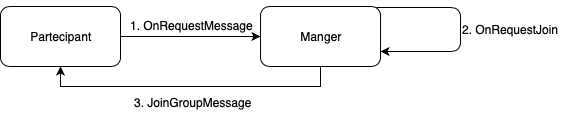
\includegraphics[width=\columnwidth]{figures/joinRequest.png}}\\%
	\caption{The graph shows the flow of execution when a participant
	wants to join an existing group}%
	\label{fig:join}%
\end{figure}
Figure \ref{fig:join} shows whenever a participant wants to join a group. First, it contacts the manager. Then, the latter elaborates the request and, eventually, it adds the new peer to the group by sending him a new \texttt{JoinGroupMsg} containing the unique ID of the new member.

The Figure \ref{fig:NewView} shows the flow of execution to instantiate a new view. Whenever a new join request or a silent crash occurs, the manager receives respectively either a \texttt{RequestJoinMsg} or a \texttt{TimeoutMsg}. Afterwords, it instantiates the view change process and, eventually, all the operational peers receives the message and execute the flush protocol. This protocol is needed to make all the participants aware that they have received all unstable messages from all the members in the group: first, every operational peer sends all the unstable messages it owns in the queue to make them stable and second,  multicasts a \texttt{FlushMsg} object indicating that they have completed the flush protocol. Only after having received the flush message from all the operational peers, a group member is allowed to install the new view.
\begin{figure}[ht]%
	\centering
	\subfloat{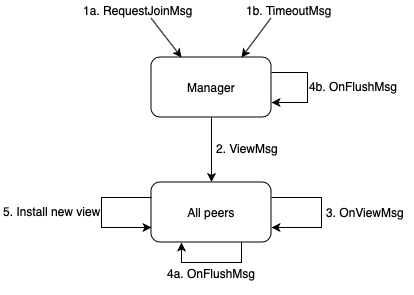
\includegraphics[width=\columnwidth]{figures/NewView.png}}\\%
	\caption{The graph shows the flow of execution when a new view has
	to be instantiated}%
	\label{fig:NewView}%
\end{figure}
In order to exchange messages, a peer has to have installed the most recent view. Simply, in the code this mechanism is handled by the \texttt{inhibit\_sends} field, which has to be zero in order to allow the exchange of messages. Every time a peer receives a view change (when the manager instantiates a new view and sends a message to each participant) the counter is incremented by one; on the other way round, each time a new view is installed, the counter is decremented.

Furthermore, the overall application tries to take into account possible delays over the channels: every message is propagated with an extremely small and random delay in order to obtain a more realistic scenario. Moreover, there are some supporting functions used to simplify the overall application: e.g., \textit{DeleteOldMessages}, \textit{FindDuplicate}, etc.

\subsection{Crash detection}
Another important scenario to be described is the silent crash detection. The implementation takes place through a simple beacon mechanism: every five seconds each peer sends a message (beacon) to the manager, indicating that specific peer is still alive. Since the channel is reliable, as soon as the manager does not receive a beacon from a participant, it can assume that the peer is crashed.

In particular, whenever a new peer joins the group, the manager schedules a timeout, implemented as a self message, 10 seconds later.  As far as the manager keeps on receiving beacons, it updates the timeout for the peer. As soon as a beacon is missing, the manager will receive its \texttt{TimeoutMsg} and it will be able to identify the crashed member. Afterwords, a new view without the crashed node is instantiated.

In particular, it is able to understand which peer crashed, thanks to a dedicated HashMap where the key-value pair is represented by the peer and a \texttt{Cancellable} object. This data structure is used to have information about the time a peer sent the beacon. By associating to each participant the event scheduled at the precise time in which the beacon was received, the group manager is able to keep track about the alive peers.





\begin{comment}
\begin{itemize}
\item describe everything you yourself did (as opposed to the fundamentals section, which explains what you built on)
\item explain the mathematical framework (if any)
\item explain your model
\item describe the developed system/algorithm/method
\end{itemize}
\end{comment}

\section{Conclusion}
This project suggests a simple implementation of a distributed application
according to the protocol. Everything works properly ad the overall system
is very easily testable thanks to the \textbf{CausalMulticast.java} class. 

\begin{comment}
	\begin{itemize}
\item summarize again what your work did, but now emphasize more the results
\item write conclusions that can be drawn from the results found and the discussion presented in the work
\end{itemize}
Again for very short documents the conclusions can be embedded with the last section, but this depends on the structure you give to your document. 

\end{comment}


\bibliographystyle{IEEEtran}
\bibliography{references}

\end{document}
